\section{Алгоритм синтаксического анализа \\ контекстно-свободного представления}

\subsection{Описание алгоритма}

// ЧЕРНОВИК

Мы пытаемся решать следующую задачу: пусть $G_1 = (N, T, S, P)$ --- произвольная КС-грамматика, $G_2$ --- NSE КС-грамматика. Алгоритм принимает на вход два рекурсивных автомата, $M_1$ и $M_2$, построенных по грамматикам $G_1$ и $G_2$ соотвественно, при этом в автомате $M_2$ левые/правые рекурсивные вызовы заменены на циклы, как в обычном конечном автомате.

Результатом работы алгоритма являются тройки вида $(X, n_1, n_2)$, где $X \in N$, $n_1, n_2$ --- номера состояний автомата $M_2$. 
Для каждой из таких троек выполняется следующее утверждение: $\exists \, \omega \in T^*$ такая, что $X \rightarrow^* \omega$ в $G_1$ и $\omega \in L(M')$, где $M'$ --- рекурсивный автомат, полученный из $M_2$ путем замены начального и конечного состояния на $n_1$ и $n_2$ соответственно.

Получая такие результаты, мы, по сути, отвечаем на вопрос о проверке пустоты пересечения КС-языка и регулярного, представленных в необычных абстракциях. 
Для КС-языка мы используем рекурсивный автомат, а для регулярного --- нечто среднее между конечным автоматом и NSE грамматикой (это нечто все еще использует стек, но только для обработки нерекурсивных вызовов). 
Такое представление эквивалентно по выразительности NSE и, следовательно, FA (см. рис. \ref{circle:lang}). 
%Но неизвестно, к какому классу сложности относится задача (и разрешима ли вообще) о проверке пустоты пересечения регулярного языка, представленного в данной форме, с КС-языком (см. рис. \ref{circle:intersec}).

%\begin{figure}[h!]
%	\begin{subfigure}[t]{0.45\textwidth}
%		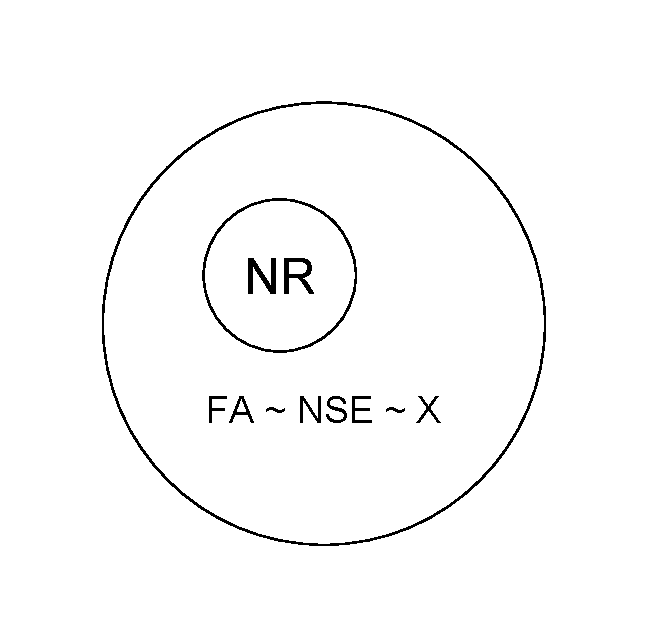
\includegraphics[width=\textwidth]{pictures/lang}
%		\caption{Выразительность языка, задаваемого абстракцией}
%		\label{circle:lang}
%	\end{subfigure}
%	~
%	\begin{subfigure}[t]{0.45\textwidth}
%		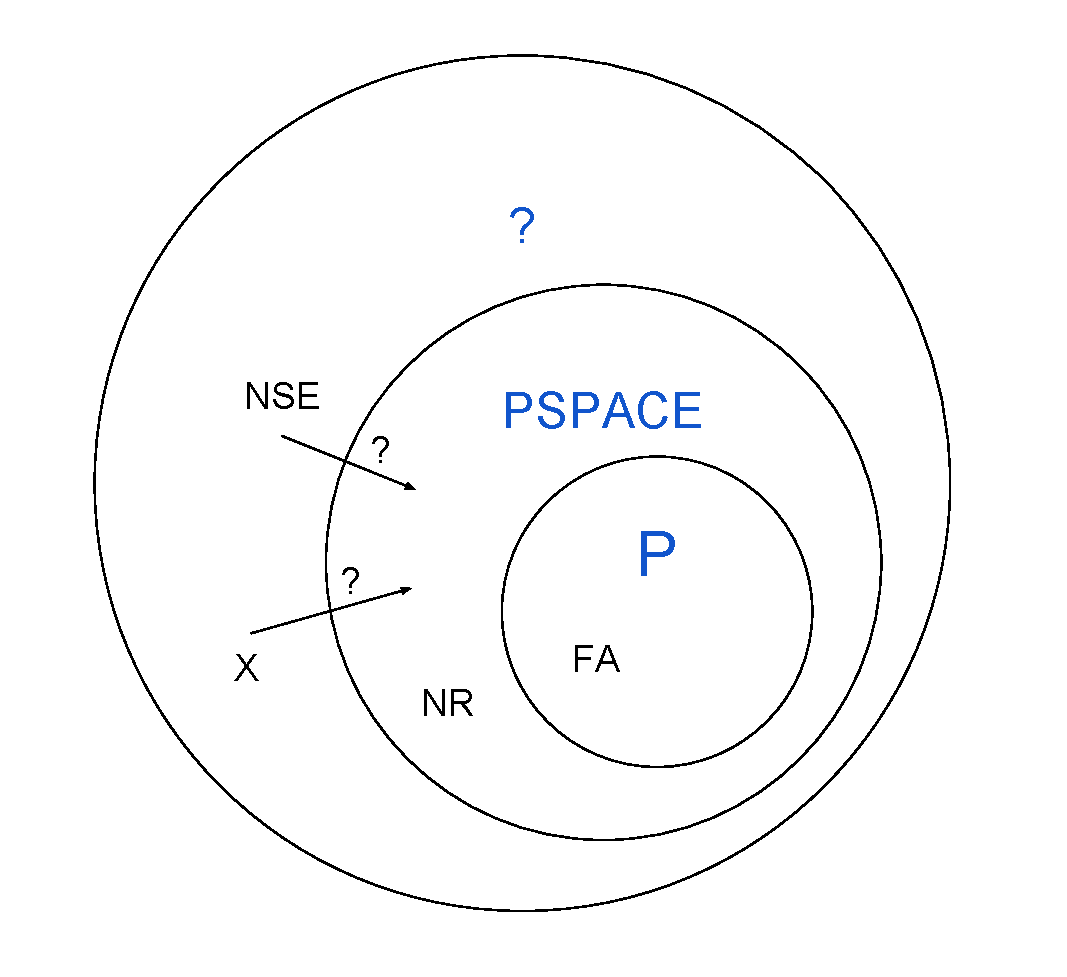
\includegraphics[width=\textwidth]{pictures/intersec_problem}
%		\caption{Класс сложности для задачи о проверке пустоты пересечения с КС-языком}
%		\label{circle:intersec}
%	\end{subfigure}
%	\caption{Красивые круги. Здесь NR --- нерекурсивная грамматика, FA --- конечный автомат, NSE --- грамматика без вложенной рекурсии, X --- наше представление}
%	\label{circle}
%\end{figure}

\subsection{Доказательство корректности}

\begin{theorem}{Завершаемость.}
	Алгоритм завершает работу за конечное число шагов для произвольных входных данных
\end{theorem}

\begin{theorem}{Корректность.}
	???
\end{theorem}